\documentclass[11pt]{article}
\usepackage{epsfig}    % to insert postscript figures
\usepackage{float}
\usepackage{listings}
\usepackage{url}
\usepackage{amsmath}
\parindent=0pt
\parskip=10pt
\begin{document}

\title{Optimal rotor arm pivot angles \\ for a collapsible drone.}
\author{ by \\ Peter Burnett and Hugh Murrell }
\maketitle

\newpage
\section*{Problem Description}

Consider the CAD drawing of the collapsible drone shown in figure \ref{fig1} below:

\begin{figure}[H]
\begin{center}
  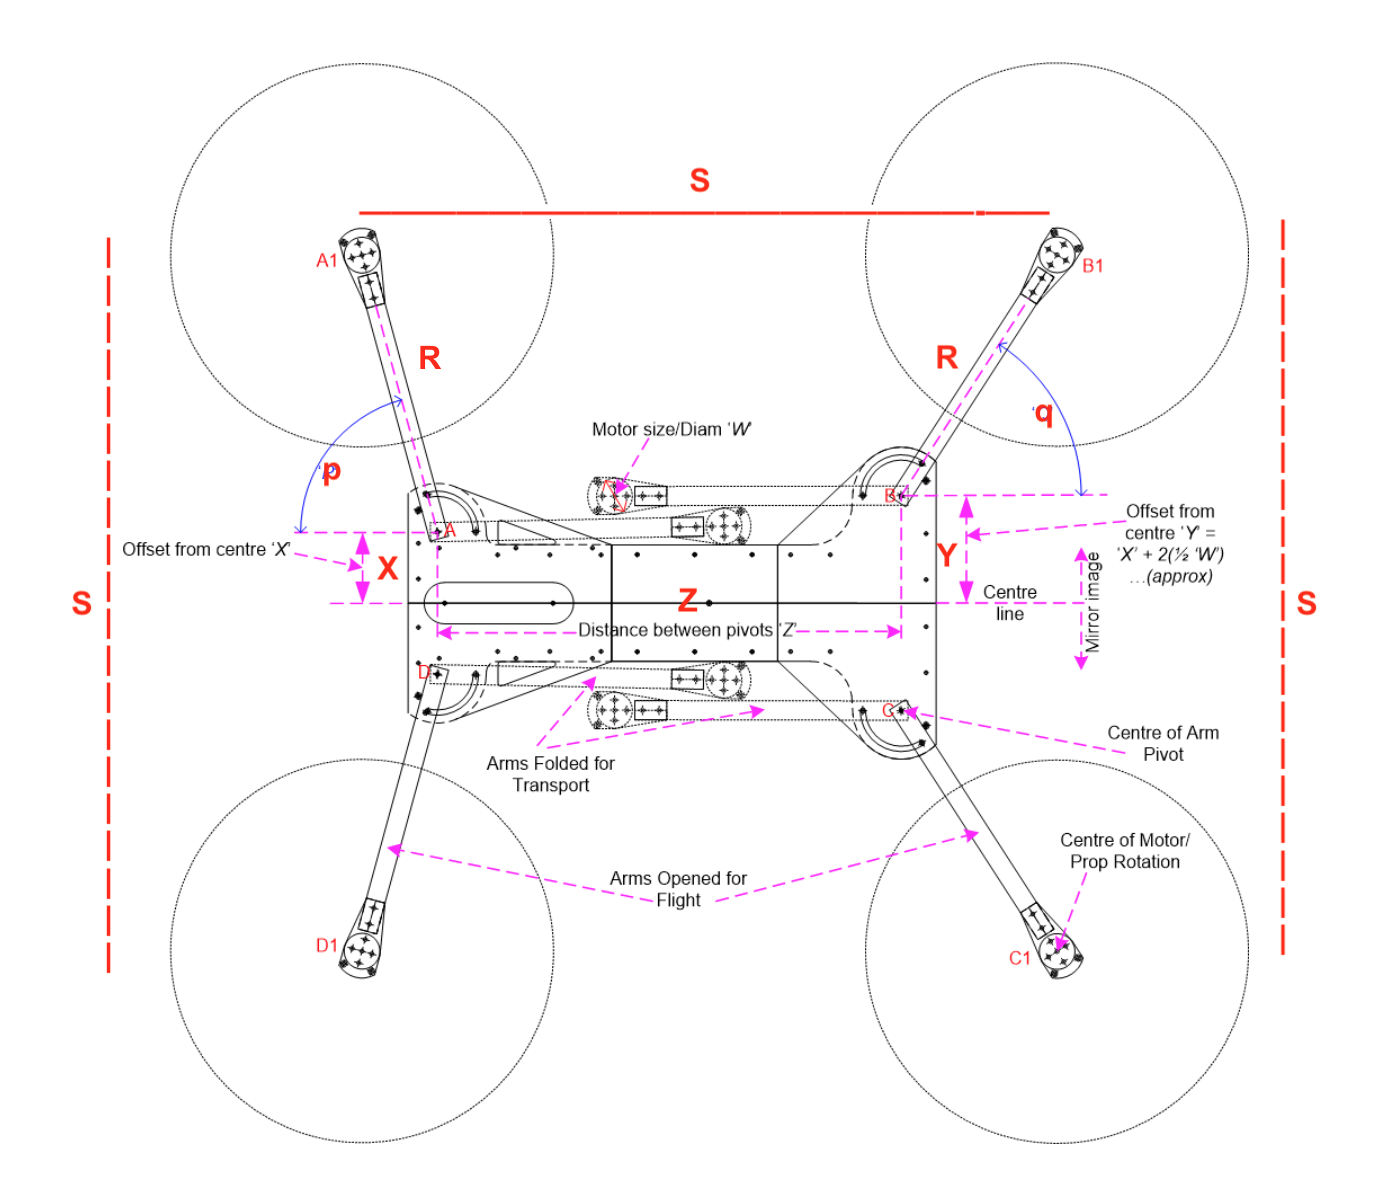
\epsfig{file=drone_drawing.png,height=3in}
\end{center}
\caption{CAD drawing of drone with collapsible arms}  
\label{fig1}
\end{figure}

In this diagram all lengths are measured in $mm$ and the annotated lengths 
are design parameters for the construction of the drone:

\begin{itemize}
\item[$R$] the length of the rotor arm (all rotor arms have the same length)
\item[$Z$] the distance between rotor arm pivot points.
\item[$X$] the offset of the front pivot arm point from the horizontal axis of symmetry.
\item[$Y$] the offset of the back pivot arm point from the horizontal axis of symmetry.
\end{itemize}

The problem is to determine the rotor arm angles, $p$ and $q$, under the
constraint that the rotor centres form a square.

\section*{Constraint Problem}

Using the constraint that the rotor centres form a square with sides of some unknown length $S$
we have:

\begin{eqnarray}
S & = & R \cos(p) + Z + R \cos(q)    \nonumber \\
S & = & 2 ( X + R \sin(p) )  \nonumber  \\
S & = & 2 ( Y + R \sin(q) )  \label{eqn1}
\end{eqnarray}

The first equation in (\ref{eqn1}) is derived from an expression for the horizontal edge of length, $S$,
whilst the last two equations are derived from expressions for the vertical front and back edges of length $S$.

The unknown edge length, $S$, can be eliminated from equations (\ref{eqn1}) yielding two non-linear
equations for the angles, $p$ and $q$ shown in equations (\ref{eqn2}) below.

\begin{eqnarray}
\cos(p) - 2 \sin(p) + \cos(q) & = & \frac{2X-Z}{R} \nonumber \\
\sin(p) - \sin(q) & = & \frac{Y-X}{R}   \label{eqn2} 
\end{eqnarray}

Although it is possible to find a closed form solution for $p$ and $q$ the calculation 
requires finding the roots of a quartic polynomial which is extremely tedious as one
can see from the Wikipedia entry \cite{quartic}.

So instead we use standard non-linear root finding technique. For example,
the {\tt scipy} python package allows us to construct the solution shown in Appendix A.

To make life easier for the reader we have also coded a {\tt javascript} solution to the
problem, this time using a numerical method called {\it Nelder-Mead} \cite{nelder}. 
The javascript code for method was lifted from an open source implementation by 
{\em Ben Frederickson} \cite{benfred}.

We also made use of the Microsoft javascript CAD library,
{\tt Maker.js} \cite{maker}, to produce drawings dependent on the user's parameter settings. 

The {\tt maker} code for the {\tt drone} scriptis given in Appendix B, but the interestedreader
can access the script from:

\small
\url{"hughmurrell.github.io/DroneDesign/maker/docs/playground/?script=drone"}.
\normalsize


\begin{thebibliography}{99}

% \bibitem{pfund} Pfund, Michele \& Fowler, J.W. \& Gupta, Jatinder. 
% {\em A survey of algorithms for single and multi-objective unrelated parallel-machine deterministic scheduling problems}. 
% Journal of the Chinese Institute of Industrial Engineers. 21. 230-241. (2004). 

\bibitem{quartic} Wikipedia Article,
{\em Quartic function} 
\url{https://en.wikipedia.org/wiki/Quartic_function}
accessed January 2021.

\bibitem{nelder} Wikipedia,
{\em The Nelder?Mead method },
\url{https://en.wikipedia.org/wiki/Nelder-Mead_method},
accessed January 2021.

\bibitem{nelder} Ben Fedrickson,
{\em fmin, unconstrained function minimization in javascript.  },
\url{https://github.com/benfred/fmin},
accessed January 2021.

\bibitem{maker} A Microsoft Garage Project,
{\em Maker.js, a JavaScript library for creating and sharing modular line drawings for CNC and laser cutters.},
\url{https://maker.js.org/},
accessed January 2021.

\end{thebibliography}

\section*{Appendix A}
\subsection*{pythod code for calculating rotor arm pivot angles}

\tiny
\begin{lstlisting}
from scipy.optimize import fsolve
from math import sin, cos, pi

def equations(vars):
    p, q = vars
    R = 225
    Z = 346
    X = 56
    Y = 84
    eq1 = cos(p) - 2*sin(p) + cos(q) - (2*X-Z)/R
    eq2 = sin(p) - sin(q) - (Y-X)/R
    return [eq1, eq2]

p, q =  fsolve(equations, (1, 1))

p = (p / pi) * 180
q = (q / pi) * 180

print(p, q)
\end{lstlisting}


\normalsize
\newpage
\section*{Appendix B}

\tiny
\begin{lstlisting}

var makerjs = require('makerjs');


// worker for nelderMead
function weightedSum(ret, w1, v1, w2, v2) {
        for (var j = 0; j < ret.length; ++j) {
            ret[j] = w1 * v1[j] + w2 * v2[j];
        }
    }


// minimizes a function using the downhill simplex method
function nelderMead(f, x0, w, parameters) {
        parameters = parameters || {};

        var maxIterations = parameters.maxIterations || x0.length * 200,
            nonZeroDelta = parameters.nonZeroDelta || 1.05,
            zeroDelta = parameters.zeroDelta || 0.001,
            minErrorDelta = parameters.minErrorDelta || 1e-6,
            minTolerance = parameters.minErrorDelta || 1e-5,
            rho = (parameters.rho !== undefined) ? parameters.rho : 1,
            chi = (parameters.chi !== undefined) ? parameters.chi : 2,
            psi = (parameters.psi !== undefined) ? parameters.psi : -0.5,
            sigma = (parameters.sigma !== undefined) ? parameters.sigma : 0.5,
            maxDiff;

        // initialize simplex.
        var N = x0.length,
            simplex = new Array(N + 1);
        simplex[0] = x0;
        simplex[0].fx = f(x0,w);
        simplex[0].id = 0;
        for (var i = 0; i < N; ++i) {
            var point = x0.slice();
            point[i] = point[i] ? point[i] * nonZeroDelta : zeroDelta;
            simplex[i+1] = point;
            simplex[i+1].fx = f(point,w);
            simplex[i+1].id = i+1;
        }

        function updateSimplex(value) {
            for (var i = 0; i < value.length; i++) {
                simplex[N][i] = value[i];
            }
            simplex[N].fx = value.fx;
        }

        var sortOrder = function(a, b) { return a.fx - b.fx; };

        var centroid = x0.slice(),
            reflected = x0.slice(),
            contracted = x0.slice(),
            expanded = x0.slice();

        for (var iteration = 0; iteration < maxIterations; ++iteration) {
            simplex.sort(sortOrder);

            if (parameters.history) {
                // copy the simplex (since later iterations will mutate)
                // sort it to have a consistent order between iterations
                var sortedSimplex = simplex.map(function (x) {
                    var state = x.slice();
                    state.fx = x.fx;
                    state.id = x.id;
                    return state;
                });
                sortedSimplex.sort(function(a,b) { return a.id - b.id; });

                parameters.history.push({x: simplex[0].slice(),
                                         fx: simplex[0].fx,
                                         simplex: sortedSimplex});
            }

            maxDiff = 0;
            for (i = 0; i < N; ++i) {
                maxDiff = Math.max(maxDiff, Math.abs(simplex[0][i] -
                                                     simplex[1][i]));
            }

            if ((Math.abs(simplex[0].fx - simplex[N].fx) < minErrorDelta) &&
                (maxDiff < minTolerance)) {
                break;
            }

            // compute the centroid of all but the worst point in the simplex
            for (i = 0; i < N; ++i) {
                centroid[i] = 0;
                for (var j = 0; j < N; ++j) {
                    centroid[i] += simplex[j][i];
                }
                centroid[i] /= N;
            }

            // reflect the worst point past the centroid
            // and compute loss at reflected point
            var worst = simplex[N];
            weightedSum(reflected, 1+rho, centroid, -rho, worst);
            reflected.fx = f(reflected,w);

            // if the reflected point is the best seen, then possibly expand
            if (reflected.fx < simplex[0].fx) {
                weightedSum(expanded, 1+chi, centroid, -chi, worst);
                expanded.fx = f(expanded,w);
                if (expanded.fx < reflected.fx) {
                    updateSimplex(expanded);
                }  else {
                    updateSimplex(reflected);
                }
            }

            // if the reflected point is worse than the second worst,
            // we need to contract
            else if (reflected.fx >= simplex[N-1].fx) {
                var shouldReduce = false;

                if (reflected.fx > worst.fx) {
                    // do an inside contraction
                    weightedSum(contracted, 1+psi, centroid, -psi, worst);
                    contracted.fx = f(contracted,w);
                    if (contracted.fx < worst.fx) {
                        updateSimplex(contracted);
                    } else {
                        shouldReduce = true;
                    }
                } else {
                    // do an outside contraction
                    weightedSum(contracted, 1-psi * rho, centroid,
                                psi*rho, worst);
                    contracted.fx = f(contracted,w);
                    if (contracted.fx < reflected.fx) {
                        updateSimplex(contracted);
                    } else {
                        shouldReduce = true;
                    }
                }

                if (shouldReduce) {
                    // if we don't contract here, we're done
                    if (sigma >= 1) break;

                    // do a reduction
                    for (i = 1; i < simplex.length; ++i) {
                        weightedSum(simplex[i], 1 - sigma, simplex[0],
                                    sigma, simplex[i]);
                        simplex[i].fx = f(simplex[i],w);
                    }
                }
            } else {
                updateSimplex(reflected);
            }
        }

        simplex.sort(sortOrder);
        return {fx : simplex[0].fx,
                x : simplex[0]};
    }

function drone(font, fontSize, R, D, Z, X, Y, P, Q){
    
    if (arguments.length === 0) {
        var defaultValues = makerjs.kit.getParameterValues(drone);
        font = defaultValues.shift();
        fontSize = defaultValues.shift();
        R = defaultValues.shift();
        D = defaultValues.shift();
        Z = defaultValues.shift();
        X = defaultValues.shift();
        Y = defaultValues.shift();
    }
    

    // compute p,q from R,Z,X,Y using nelderMead
    function loss(x,w) {
        var p = x[0], q = x[1];
        var R = w[0], Z = w[1], X = w[2], Y = w[3];
        var f1 = Math.cos(p) - 2 * Math.sin(p) + Math.cos(q) - (2*X-Z)/R;
        var f2 = Math.sin(p) - Math.sin(q) - (Y-X)/R;
        return Math.abs(f1) + Math.abs(f2);
    }

    var solution = nelderMead(loss, [0.786, 0.786], [R,Z,X,Y]);
     
    p = solution.x[0];
    q = solution.x[1];
                                    
    console.log("user selected:");
    console.log("R = "+R);
    console.log("D = "+D);
    console.log("X = "+X);
    console.log("Y = "+Y);
    console.log("computed:");
    console.log("P = " + p*180/Math.PI);
    console.log("Q = " + q*180/Math.PI);
    
    var cp=R*Math.cos(p);
    var sp=R*Math.sin(p);
    var cq=R*Math.cos(q);
    var sq=R*Math.sin(q);
    
    var top_dots = [
                    [0, X + sp],
                    [cp,X],
                    [cp,0],
                    [cp+Z,0],
                    [cp+Z,Y],
                    [cp+Z+cq,Y+sq]
                    ];
    
    var top_drone = new makerjs.models.ConnectTheDots(true, top_dots);
    
    var bot_dots = [
                    [0, -(X + sp)],
                    [cp,-X],
                    [cp,0],
                    [cp+Z,0],
                    [cp+Z,-Y],
                    [cp+Z+cq,-(Y+sq)]
                    ];
    
    var bot_drone = new makerjs.models.ConnectTheDots(true, bot_dots);
    
    
    var rotors = {
    paths: {
        "ft": new makerjs.paths.Arc([0, X + sp], D/2, 0, 360),
        "fb": new makerjs.paths.Arc([0, -(X + sp)], D/2, 0, 360),
        "bt": new makerjs.paths.Arc([cp+Z+cq,Y+sq], D/2, 0, 360),
        "bb": new makerjs.paths.Arc([cp+Z+cq,-(Y+sq)], D/2, 0, 360)
        }
    };
                                                                                                                        
    var ovr = Math.abs((Y-X)/2);
                       
    var rot=(Math.PI-p)*180/Math.PI;
    var arm_ft = new makerjs.models.Oval(R+2*ovr, 2*ovr);
    makerjs.model.move(arm_ft,[cp-ovr,X-ovr]);
    makerjs.model.rotate(arm_ft,rot,[cp,X]);
                                        
    rot=(q)*180/Math.PI;
    var arm_bt = new makerjs.models.Oval(R+2*ovr, 2*ovr);
    makerjs.model.move(arm_bt,[cp+Z-ovr,Y-ovr]);
    makerjs.model.rotate(arm_bt,rot,[cp+Z,Y]);
                                
    rot=(Math.PI+p)*180/Math.PI;
    var arm_fb = new makerjs.models.Oval(R+2*ovr, 2*ovr);
    makerjs.model.move(arm_fb,[cp-ovr,-X-ovr]);
    makerjs.model.rotate(arm_fb,rot,[cp,-X]);
                        
    rot=(-q)*180/Math.PI;
    var arm_bb = new makerjs.models.Oval(R+2*ovr, 2*ovr);
    makerjs.model.move(arm_bb,[cp+Z-ovr,-Y-ovr]);
    makerjs.model.rotate(arm_bb,rot,[cp+Z,-Y]);
            
    var cas_tf = new makerjs.models.Oval((2*Z/3)+2*ovr, 2*ovr);
    makerjs.model.move(cas_tf,[cp-ovr,X-ovr]);
                        
    var cas_tb = new makerjs.models.Oval((2*Z/3)+2*ovr, 2*ovr);
    makerjs.model.move(cas_tb,[cp+Z-ovr,Y-ovr]);
    makerjs.model.rotate(cas_tb,180,[cp+Z,Y]);
                            
    var cas_bf = new makerjs.models.Oval((2*Z/3)+2*ovr, 2*ovr);
    makerjs.model.move(cas_bf,[cp-ovr,-X-ovr]);
            
    var cas_bb = new makerjs.models.Oval((2*Z/3)+2*ovr, 2*ovr);
    makerjs.model.move(cas_bb,[cp+Z-ovr,-Y-ovr]);
    makerjs.model.rotate(cas_bb,180,[cp+Z,-Y]);
                                          
    var p_annotate = new makerjs.models.Text(font,
            "P = " + (p*180/Math.PI).toFixed(1), fontSize, false, false);
    makerjs.model.move(p_annotate,[cp-ovr-(7*fontSize),0]);
                      
    var q_annotate = new makerjs.models.Text(font,
            "Q = " + (q*180/Math.PI).toFixed(1), fontSize, false, false);
    makerjs.model.move(q_annotate,[cp+Z+(2*fontSize),0]);
                      
    var z_annotate = new makerjs.models.Text(font,
            "Z = " + Z, fontSize/2, false, false);
    makerjs.model.move(z_annotate,[cp+Z/2-(2*fontSize/2),fontSize/4]);
            
    var r_annotate = new makerjs.models.Text(font,
            "R = " + R, fontSize/2, false, false);
    makerjs.model.move(r_annotate,[cp+Z+(2*fontSize/2),Y+fontSize/4]);
                                   
    var y_annotate = new makerjs.models.Text(font,
            "Y = " + Y, fontSize/2, false, false);
    makerjs.model.move(y_annotate,[cp+Z+(1*fontSize/2),-Y/2]);
                                         
    var x_annotate = new makerjs.models.Text(font,
            "X = " + X, fontSize/2, false, false);
    makerjs.model.move(x_annotate,[cp+(1*fontSize/2),-X/2]);
                                   
    var d_annotate = new makerjs.models.Text(font,
            "D = " + D, fontSize/2, false, false);
    makerjs.model.move(d_annotate,[D/2+(1*fontSize/2),-Y-sp+fontSize]);
            
    this.models = {
            "top": top_drone,
            "bottom": bot_drone,
            "rotor blades": rotors,
            "arm_ft": arm_ft,
            "arm_bt": arm_bt,
            "arm_fb": arm_fb,
            "arm_bb": arm_bb,
            "cas_tf": cas_tf,
            "cas_tb": cas_tb,
            "cas_bf": cas_bf,
            "cas_bb": cas_bb,
            "p_annotate": p_annotate,
            "q_annotate": q_annotate,
            "z_annotate": z_annotate,
            "r_annotate": r_annotate,
            "y_annotate": y_annotate,
            "x_annotate": x_annotate,
            "d_annotate": d_annotate
        };

}

                                          
    drone.metaParameters = [
        { title: "font", type: "font", value: '#stencil' },
        { title: "font size", type: "range", min: 10, max: 200, value: 48 },
        { title: "R", type: "range", min: 50, max: 400, value: 225 },
        { title: "D", type: "range", min: 10, max: 300, value: 200 },
        { title: "Z", type: "range", min: 100, max: 900, value: 346 },
        { title: "X", type: "range", min: 10, max: 100, value: 56 },
        { title: "Y", type: "range", min: 40, max: 150, value: 84 }
     ];
                           


    module.exports = drone;

\end{lstlisting}





\end{document}


